\chapter{Scrum}
\section{Introduction to Scrum}

\par{
Scrum is originally a tactic used in rugby. All players are gathered around the ball, holding each other and trying to be the first team to get the ball. Scrum is applied when an error was made or a ball was put out of game. The scrum methodology is an applied software team management philosophy following the same principle. It is agile and therefore an ideal example for an applied agile methodology. 
\par{
Scrum not only tries to avoid errors like the "tunnel development", "contract gaming", "squirrel burgers" or working with the "magic toolbox" but it also enforces a game like style in design and implementation of Software. A Scrum team is considered very transparent and flexible, giving always clear information about the current state of the development. 
}
\par{
Main goal is to generated measurable value increments after each step in the development of software, by minimizing the time between each working increment of the software.
}
\section{Scrum Principles and elements}
\subsection{Radiator, stories, backlog and sprints}
\par{
The center piece of scrum is a big chart showing the overview of all currently developed features. This chart is called the radiator while the features are called stories. A story is comparable to a specific feature. Each described as a use-case and containing an estimation in time or points for the completion. Those information are written on a post-it and put on the radiator. 
}
\par{
The radiator does not only show the current stories but all stories, whether they are completed, in progress or in the backlog. The radiator also contains a chart summing up the current points in progress, the points already used and the remaining points. This chart is called a burn-down diagram. This gives an always-up-to-date overview of the current state of the project and is visible to anyone working on the project. 
}
\par{
Another element are the sprints. They are time frames set to finish the next set of stories. Stories assigned to a project are stored in the sprint-backlog. All stories assigned to the team are stored in the product backlog. 
}
\begin{figure}[h!]
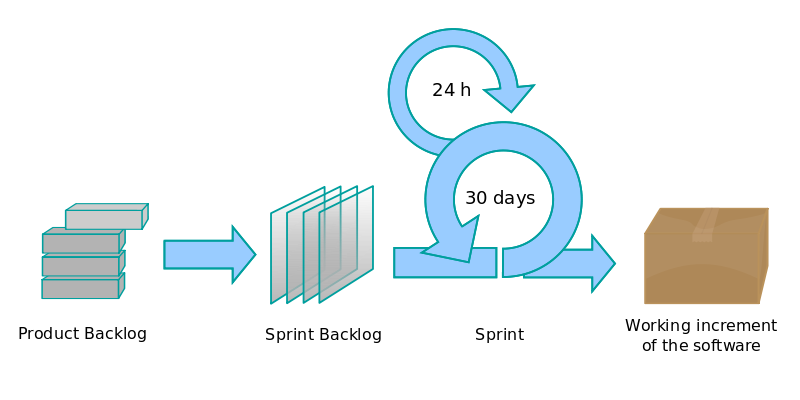
\includegraphics[width=\textwidth]{scrum_process.png}
\caption{\label{scrumproc}Illustration of the scrum process}
\end{figure}

\subsection{Roles}
\textbf{product-owner}
\par{
The most important role in Scrum is the product-owner. He is responsible to present new stories and priories them. He is the manager behind the backlog and directs the team to fulfill the goals set by the stakeholders. 
}
\\\\
\textbf{scrum-master}
\par{
Takes over the role of a mentor and guide to apply the scrum rules. He controls the teams and leads discussion and meetings. He is not to be confused with the product-owner as a scrum-master does not manage the team, but only leads it. He can be compared to the coach. A Scrum master protects the teams from any influence and helps focusing on the tasks ahead.
}
\\\\
\textbf{developer-team}
\par{
Of course every team needs grunts for the work. Developer take over the role as designer and developer. They follow instructions and are organized as teams. Each team focusing on the same stories.
}
\\\\
\textbf{stakeholders}
\par{
Stakeholders are the customers. They provide feedback to the product-owner and provide the income. They are only involved in the sprint meetings. 
}
\\\\
\textbf{management}
\par{
The management has no special function but to provide stakeholders (Marketing) and deliver a work environment for the developer teams (Facility Manager, HR Manager). 
}
\subsection{Meetings}
\subsubsection{Daily Scrums}
\par{
Daily meeting used to check on work progress. Therefore it is discussed what changed since last meeting and what is up ahead. Those meetings are timeboxed to 15 minutes.
}
\subsubsection{Backlog grooming}
\par{
A meeting done during a sprint. The current stories are updated and new stories are optimized using techniques like planning poker. After such a meeting the backlog is re estimated providing sharper estimation of project state.
}
\subsubsection{Scrum of Scrums}
\par{
Meeting of team or clusters of teams to discuss overlapping stories or common work. Usually after a daily scrum.
}
\subsubsection{Sprint planning meeting}
\par{
Meeting before the start of a sprint to fix the backlog.
}
\subsubsection{End of cycle}
\par{
Meeting at the end of a sprint to discuss the sprint in retrospective. This can be seen as an after action review or a debriefing. 
}